\newpage
\hypertarget{uploading-to-uva-online-judge}{%
\mysection{Uploading to UVA Online Judge}\label{uploading-to-uva-online-judge}}

\begin{quote}
Adapted from Zachary Kingcades tutorial.
\end{quote}

\hypertarget{overview}{%
\mysubsection{Overview}\label{overview}}

There is a little different angle we must take when writing code to be
uploaded to https://onlinejudge.org/. Just like I have stressed in class
(oh remember the days when we had class \ldots) having a base knowledge
of the use of the command line can be beneficial. This tutorial will
discuss a couple of those skills and prepare you for uploading code to
UVA Online judge.

Keep in mind that solving these types of problems isn't just for
competition, its relevant for school and especially as a prep for
interviewing.

\hypertarget{registration-and-overview}{%
\mysubsubsection{Registration and Overview}\label{registration-and-overview}}

Onlinejudge has thousands of problems to browse and solve. You can look
at them without registering, but you will need to register to submit
solutions so go ahead and do that
\href{https://onlinejudge.org/index.php?option=com_comprofiler\&task=registers}{HERE}.

The major portion of Onlinejudge is its
\href{https://uhunt.onlinejudge.org/}{uHunt} section. This is where you
browse problems, submit your solutions, see statistics about each
problem, see latest submissions, and most importantly where you see the
status of your own submissions. You can click on the link I provided,
\textbf{or} look for this icon on the main page:

\begin{center}

\includegraphics[scale=.4]{images/uva_icon_sp_2020.png}\\
\end{center}

\hypertarget{selecting-a-problem}{%
\mysubsubsection{Selecting A Problem}\label{selecting-a-problem}}

You're registered, and ready to solve problems! How do you pick a
problem? There are many different ways and reasons to select a problem.

We are solving problems that require the understanding of specific data
structures as well as problem solving paradigms. Data structures
include: lists, arrays, stacks, queues, trees, graphs along with
variants or combos of each. Problem Solving Paradigms include: brute
force, divide and conquer, greedy, and dynamic programming.

We will use Competitive Programming 3 to help us choose problems that
will best be solved by choosing the proper data structure accompanied
with the correct problem solving paradigm.

\begin{quote}
\textbf{Note 1:} I hate stealing from any author, especially one who
created such a great resource. I'm sure he would understand our dilemma
this semester. I bought my own copy, and would encourage all of you to
\href{https://cpbook.net/\#CP3details}{purchase a copy}. Its a great
programming resource since it really concentrates on problem solving in
general, not just competitive programming.
\end{quote}

\begin{quote}
\textbf{Note 2:} The only reason I haven't used this from the beginning
is \ldots{} cheating :( You can find most of the solutions online. Even
though I have a defense for this, its just exhausting. More later
\ldots{}
\end{quote}

You don't only have to choose problems based on data structures and problem solving paradigms, believe it or not, people actually solve these for fun! I would recommend you solve as many of these as you have time for in addition to your course work. Lots of solutions will pad your resume` AND prepare you for interviews. So how do you choose problems to solve if its not for specific data structures? You can choose based on difficulty and how cool the name is. To do this, you have to \href{https://onlinejudge.org/index.php?option=com_onlinejudge\&Itemid=8}{browse} the problem sets. Below is the first menu of problems to choose from. We will concentrate on the two sets I placed a box around:

\begin{center}
\includegraphics[scale=.4]{images/brows_problems_sp_2020.png}
\end{center}

% \href{https://onlinejudge.org/index.php?option=com_onlinejudge\&Itemid=8}{\includegraphics[width=5.20833in,height=\textheight]{https://cs.msutexas.edu/~griffin/zcloud/zcloud-files/brows_problems_sp_2020.png}}

As you click folders, they drill down into other folders and finally lists of problems. If you drill down into any of the folders you will end up seeing something similar to below:

\begin{center}
\includegraphics[scale=.4]{images/problem_difficulty_sp_2020.png}
\end{center}

% \href{https://onlinejudge.org/index.php?option=com_onlinejudge\&Itemid=8\&category=6}{\includegraphics[width=5.20833in,height=\textheight]{https://cs.msutexas.edu/~griffin/zcloud/zcloud-files/problem_difficulty_sp_2020.png}}

We can see in a brief glance that lots of "red" = hard, and lots of "green" = easy (generally). The left column shows how many total submissions vs how many solved. In other words, lots of red means it takes many submissions before someone gets it correct. The right column is percentage of people that attempted the problem actually solved it. So, if you want an easy problem, find one that has a left column with 90+ solution percentage.

If you need to find a specific problem, they all have numbers (the ones we will use). So you can go \href{https://onlinejudge.org/index.php?option=com_onlinejudge\&Itemid=8}{browse} and find problems using the number to navigate folders, or you can go to \href{https://uhunt.onlinejudge.org/}{uHunt} and put the number in a search form (see \#1 on image).

\begin{center}
\includegraphics[scale=.4]{images/uhunt_browse_problems.png}
\end{center}

% \includegraphics[width=5.20833in,height=\textheight]{https://cs.msutexas.edu/~griffin/zcloud/zcloud-files/uhunt_browse_problems.png}

This will bring up a link to the problem description (see \#2 on image) which you can download and keep as a  reference as your solving. It also give you basic stats and current ``whats going on'' with the problem (see \#3 on image).

To stay organized I typically create a folder with the problem number as the folder name, and save everything from that associated problem in there. There will always be the pdf for the problem, multiple data sets to test your problem, and the actual source code. So, organizing with folders and problem numbers is recommended.

Aside from being organized and trying to decide what problems to solve, you really just need to break the ice and get a solution uploaded to uHunt. So lets start with a super easy one called \texttt{11172\ -\ Relational\ Operator}

\hypertarget{solving-a-problem}{%
\mysubsubsection{Solving A Problem}\label{solving-a-problem}}

You can refer to the previous section and go get the pdf of the problem we will solve. Its number is "11172". But for this tutorial, here are the contents:

\begin{center}\rule{0.5\linewidth}{0.5pt}\end{center}

\hypertarget{relational-operator}{%
\mysubsubsection{11172 - Relational Operator}\label{relational-operator}}

\begin{quote}
Time limit: 3.000 seconds
\end{quote}

Some operators checks about the relationship between two values and
these operators are called relational operators. Given two numerical
values your job is just to find out the relationship between them that
is (i) First one is greater than the second (ii) First one is less than
the second or (iii) First and second one is equal.

\hypertarget{input}{%
\paragraph{Input}\label{input}}

First line of the input file is an integer
\texttt{t\ (t\ \textless{}\ 15)} which denotes how many sets of inputs
are there. Each of the next \texttt{t} lines contain two integers
\texttt{a} and \texttt{b}
\texttt{(\textbar{}a\textbar{},\ \textbar{}b\textbar{}\ \textless{}\ 1000000001)}.

\hypertarget{output}{%
\paragraph{Output}\label{output}}

For each line of input produce one line of output. This line contains
any one of the relational operators \texttt{\textgreater{}},
\texttt{\textless{}} or \texttt{=}, which indicates the relation that is
appropriate for the given two numbers.

\hypertarget{sample-input}{%
\paragraph{Sample Input}\label{sample-input}}

\begin{verbatim}
3
10 20
20 10
10 10
\end{verbatim}

\hypertarget{sample-output}{%
\paragraph{Sample Output}\label{sample-output}}

\begin{verbatim}
<
>
=
\end{verbatim}

\begin{center}\rule{0.5\linewidth}{0.5pt}\end{center}

\hypertarget{coding-the-problem}{%
\mysubsubsection{Coding The Problem}\label{coding-the-problem}}

\hypertarget{start}{%
\paragraph{Start}\label{start}}

You should read over the problem and start to formulate a solution by
breaking it down into manageable components (more later). This problem
is easy. I will say, however, that initially none of the problems
\textbf{read} easy. They use mathematical notation to remove ambiguity
from the problem definition, and it is a bit confounding at first.
However it simply requires a little practice or a nice \textbf{slow}
approach to absorb its meaning.

\hypertarget{think}{%
\paragraph{Think}\label{think}}

For each problem we recommend that you THINK about it, re-read it, then
start your solution on paper. Also, when solving these problems, always
look at the limits as described in the problem
(e.g.~\texttt{t\ \textless{}\ 15} and
\texttt{(\textbar{}a\textbar{},\ \textbar{}b\textbar{}\ \textless{}\ 1000000001)}).
These could have an impact on the solution. For example, does
\texttt{1000000001} fit in an integer data type? Or should it be long?
Int works when uploaded for this solution, but on a tougher problem this
could bite you in the butt.

\hypertarget{code}{%
\paragraph{Code}\label{code}}

After you come up with a proposed solution, start to code it. Normal
coding conventions that we stress in class are a little out the window.
\textbf{Not all}, but some. Rules like self documenting variable names,
comments for each variable, organized procedural solution (lots of
functions) are all relaxed for these solutions.

\hypertarget{nuances}{%
\paragraph{Nuances}\label{nuances}}

Also, we want all the little speedups we can manage. \textbf{Example 1)}
in larger solutions where a function seems appropriate, you may want to
keep your code in main (inline), a function call is ever so slightly
slower than inline code. \textbf{Example 2)} Another miniscule speedup
is something as simple as re-defining \texttt{endl} to
\texttt{\textbackslash{}n}. The first one is interpreted as a newline
\textbf{AND} a flush of the output buffer. If one of the problems you
are solving has you writing to standard out thousands and thousands of
times, the extra flush may slow you down. Both of these are tiny little
speedups, but put a lot of those tiny speedups together, and it could
make a difference. Difference in what you ask? The first line after the
title in our problem statement states:
\texttt{Time\ limit:\ 3.000\ seconds}. That's the problem. Each solution
has a time limit to complete.

\hypertarget{stdin}{%
\paragraph{Stdin}\label{stdin}}

Lastly \textbf{cin} is NOT being used to prompt a user for input. It is
being used to read from an input file! Jump below the code and input
file \ldots{}

\begin{minted}[]{c++}
#include <iostream>

#define endl "\n"

using namespace std;

int  main(){
    int c,l,r,i=0;
    cin>>c;
     while(i<c){
         cin>>l>>r;
         if(l<r){
             cout<<'<'<<endl;
         }else if(l>r){
             cout<<'>'<<endl;
         }else{
             cout<<'='<<endl;
         }
         i++;
     }
     return 0;
}
\end{minted}


\hypertarget{infile}{%
\paragraph{infile}\label{infile}}

\begin{verbatim}
3
10 20
20 10
10 10
\end{verbatim}

\textbf{cin} reads from
\href{https://en.wikipedia.org/wiki/Standard_streams}{stdin} which means
a default connected stream for whatever platform you are on. Typically
when you run a program, and you need input, you pause execution of the
program with a \texttt{cin} and then it waits for input from the
``keyboard''. And when you write using \texttt{cout} it writes to
\texttt{stdout} which is usually the terminal (or dos window). As a side
note there is also \texttt{stderr} which is where errors are directed to
(we don't deal with stderr, as its usually used with log files and
such).

We change \texttt{stdin} to be input from a file. Why? If you upload
your code to be auto run, how do you process a file? You could be given
a path and a file name, but its actually easier to redirect a file into
your program.

Given:

\begin{itemize}
\tightlist
\item
  code is in \texttt{main.cpp}
\item
  we compile and its executable is now \texttt{main.exe}
\item
  we have an input file called \texttt{infile}
\end{itemize}

We can read \texttt{infile} using \texttt{cin} by doing:

\begin{verbatim}
./main.exe < infile 
\end{verbatim}

The command above says to take \texttt{infile} and send it into
\texttt{main.exe} as if we opened it, except we can use \texttt{cin} to
read from it. Basically, we changed \texttt{stdin} to be a file, instead
of the keyboard.

If you refer back to the code snippet, and infile, - line 9 reads in the
3, telling us how many ``pairs'' of values we need to read. - line 11
then reads in two values for every iteration of the loop

\hypertarget{run-in-visual-studio}{%
\mysubsubsection{Run in Visual Studio :(}\label{run-in-visual-studio}}

You have to edit the projects properties. So whichever side your
solution explorer is:

\begin{itemize}
\tightlist
\item
  Right Click on the Project and select Properties.
\item
  Project -\textgreater{} Properties -\textgreater{} Debugging
  -\textgreater{} Command Arguments
\item
  Add the following to your Command Arguments:
  \texttt{\textless{}\ input.txt}
\item
  Or something like that
\end{itemize}

\hypertarget{run-in-terminal}{%
\mysubsubsection{Run in Terminal}\label{run-in-terminal}}

A better way is to use command line and a bash console like
\texttt{gitbash}.

\begin{itemize}
\tightlist
\item
  Change into your folder with your code and input file.
\item
  Compile:

  \begin{itemize}
  \tightlist
  \item
    \texttt{g++\ \textless{}filename\textgreater{}\ -o\ \textless{}executablename\textgreater{}}
  \item
    \texttt{g++\ main.cpp\ -o\ main}
  \end{itemize}
\item
  Run:

  \begin{itemize}
  \tightlist
  \item
    \texttt{./main\ \textless{}\ inputfile}
  \end{itemize}
\end{itemize}

If you use any of the c++11 or later code constructs you will need to
set the compiler standard when compiling:

\begin{itemize}
\tightlist
\item
  Compile:

  \begin{itemize}
  \tightlist
  \item
    \texttt{g++\ -std=c++17\ main.cpp\ -o\ main}
  \item
    or replace c++17 with c++11 if thats what you need
  \end{itemize}
\end{itemize}

\hypertarget{repl.it}{%
\mysubsubsection{Repl.it}\label{repl.it}}

Repl.it is kinda awesome. Yes I said it. They give us a pretty nice
virtual linux environment to run our programs in. Basically, they give
us a virtual machine / command line solution \ldots{} in the browser. I
have the example from above here:
https://repl.it/{@rugbyprof/stdinexample}. Even if you don't have an
account it will let you run and edit that code. I would recommend
creating an account. Here is a tutorial on creating and using repl.it:
https://cs.msutexas.edu/replit\_tutorial/

\hypertarget{start-1}{%
\paragraph{Start}\label{start-1}}

\begin{itemize}
\tightlist
\item
  Click run so that it ``compiles'' first time.
\item
  You will have to stop it (see next pic)
\end{itemize}


\begin{center}
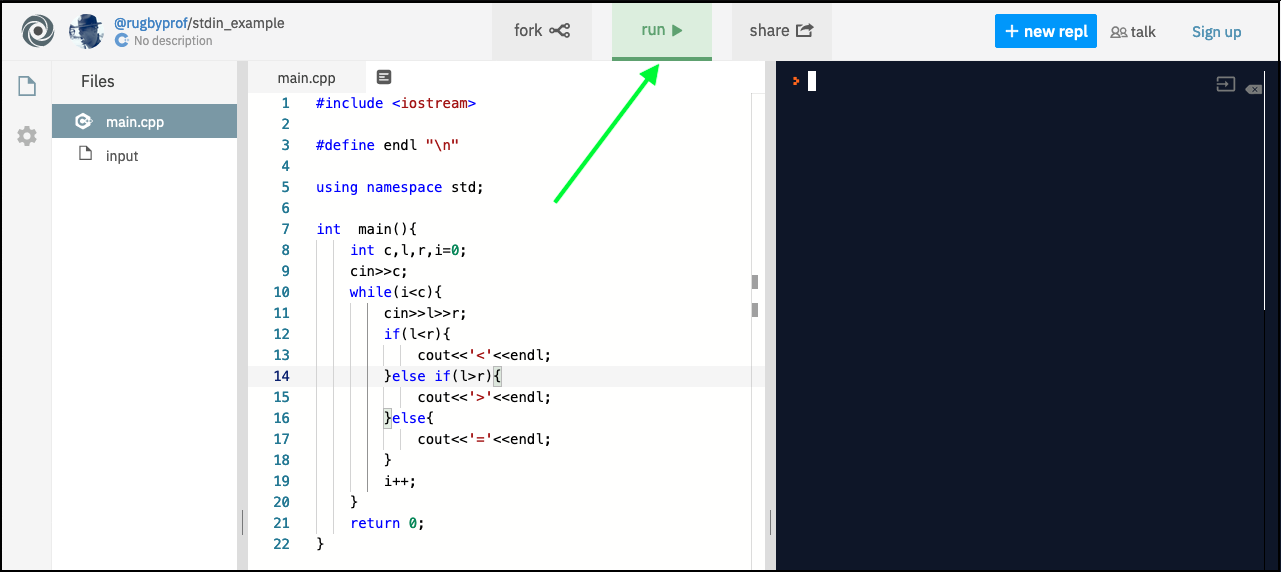
\includegraphics[scale=.4]{images/replit_stdin_1.png}
\end{center}

\hypertarget{stop}{%
\paragraph{Stop}\label{stop}}

\begin{itemize}
\tightlist
\item
  It will not finish, since its waiting for input:)
\item
  \texttt{cin} is still defined to read keyboard input, so hit the stop
  button.
\item
  You should see \texttt{exited,\ terminated} in the terminal.
\end{itemize}

\begin{center}
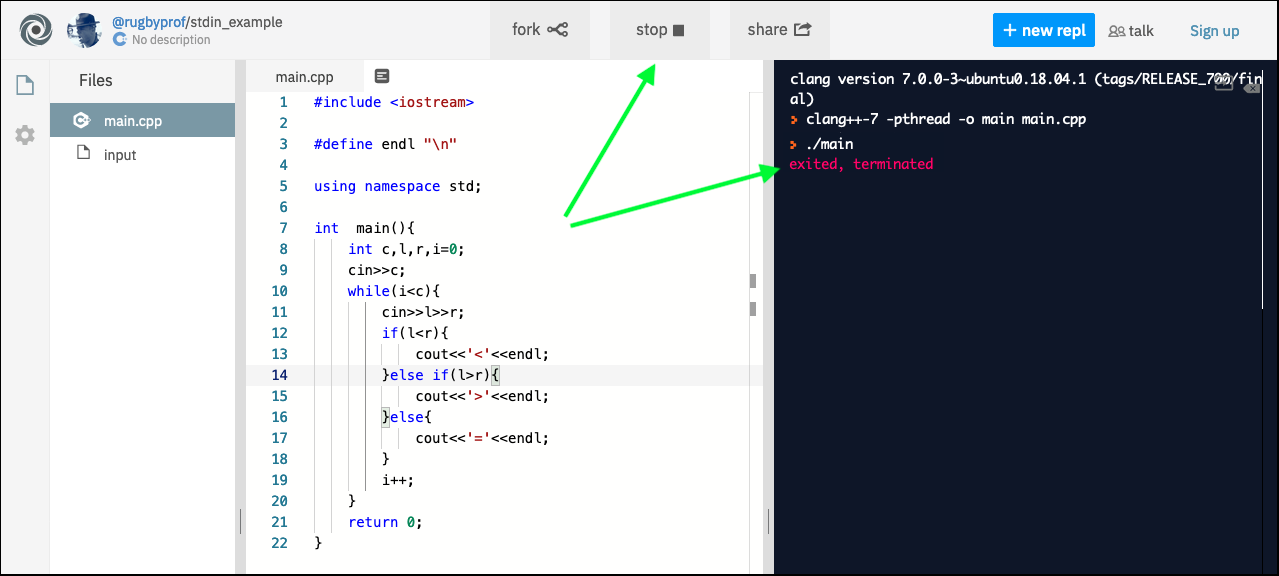
\includegraphics[scale=.4]{images/replit_stdin_2.png}
\end{center}

\hypertarget{test-run}{%
\paragraph{Test Run}\label{test-run}}

\begin{itemize}
\tightlist
\item
  When we hit ``run'' the first time , Replit compiled our code and made
  an executable with the same name as our file (minus the extension).
\item
  Since Replit is a linux virtual machine, we can run our program from
  the provided command line!
\item
  So, you can type \texttt{./main\ \textless{}\ input} in the terminal
  and get a correct run (notice we have output in the green box).
\end{itemize}

\begin{center}
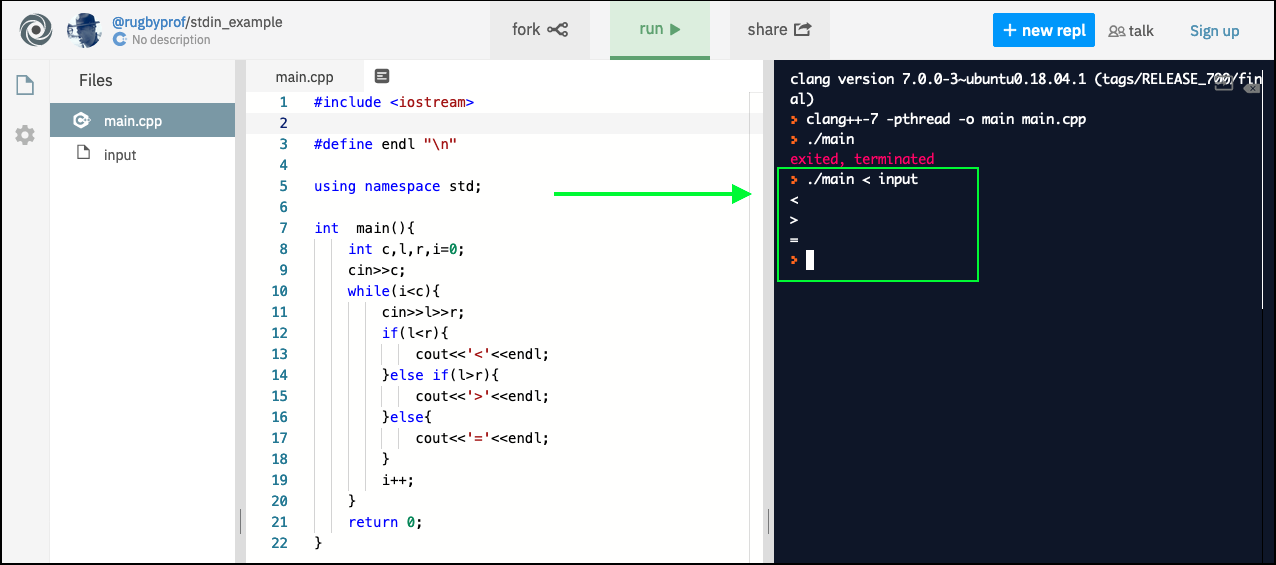
\includegraphics[scale=.4]{images/replit_stdin_3.png}
\end{center}

\hypertarget{compile}{%
\paragraph{Compile}\label{compile}}

\begin{itemize}
\tightlist
\item
  We don't want to have to hit ``run'' to get a new executable every
  time we make a change to our source code. And we don't have to.
\item
  Again, Replit gives us a linux terminal, so let us compile our own
  code using the terminal they so nicely gave us.
\item
  So as you are testing your code, you can use the \texttt{up\ arrow} to
  cycle through the necessary commands (after you have typed them at
  least once).

  \begin{itemize}
  \tightlist
  \item
    Make a change, then using the terminal:
  \item
    Compile: \texttt{g++\ main.cpp\ -o\ main}
  \item
    Run: \texttt{./main\ \textless{}\ input}
  \end{itemize}
\end{itemize}

\begin{center}
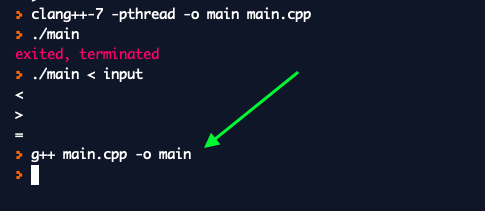
\includegraphics[scale=.4]{images/replit_stdin_5.png}
\end{center}

\hypertarget{testing-your-solution}{%
\mysubsubsection{Testing Your Solution}\label{testing-your-solution}}

You can now run your code using an input file as stdin. But how do we
know if the solution is correct? You know its correct if:

\begin{itemize}
\tightlist
\item
  You thought of every edge case possible.
\item
  You incorporated all nuances of the problem description into your
  solution.
\item
  Your output is formatted perfectly.
\item
  You are smarter than anyone you know.
\end{itemize}

The problem is, you really do not know if your solution is correct. You
can upload it to uHunt and roll the dice to see if your solution will be
accepted. Or, you can try to ensure your solution is correct by running
multiple test data sets.

If you go to the problems page where you got the pdf from, you will see
a lady bug at the top right above the problem statement. Click on it. It
will take you from
\href{https://onlinejudge.org/index.php?option=com_onlinejudge\&Itemid=8\&category=24\&page=show_problem\&problem=2113}{uHunt}
to \href{https://www.udebug.com/UVa/11172}{uDebug} where you have some
options for testing your solution more thoroughly using data sets
uploaded by other users. They go way beyond the example data given in
the problem, and will help you determine if you really did thing about
all the ``edge cases'' that might appear in the data.

\hypertarget{go-debug}{%
\paragraph{Go Debug}\label{go-debug}}


\begin{center}
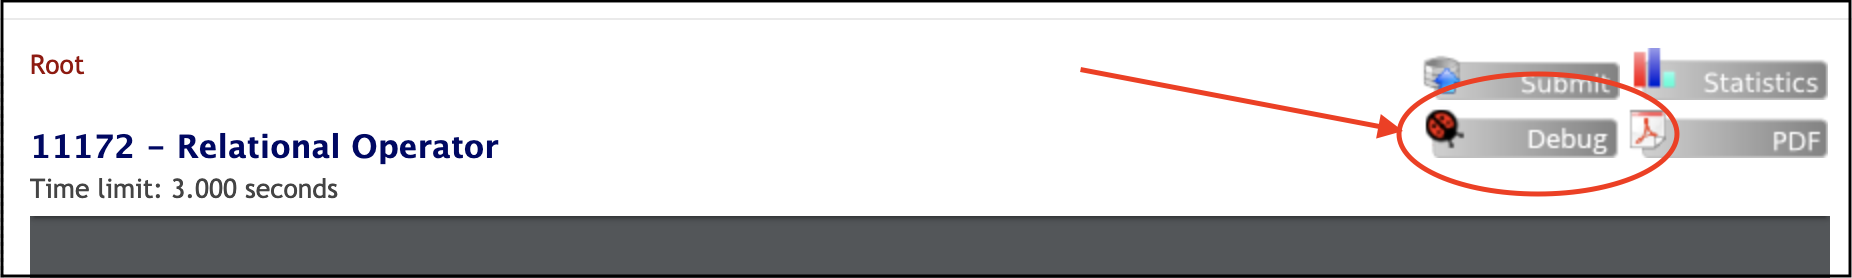
\includegraphics[scale=.4]{images/replit_debug_sp_2020.png}
\end{center}

\hypertarget{getting-data}{%
\paragraph{Getting Data}\label{getting-data}}

\begin{itemize}
\tightlist
\item
  When you go to the debug site for your problem, you will see multiple
  data sets to choose from as I enclosed in a box.
\item
  Above the blue box, you will see a link to the most popular input
  data. But all of them should help you debug.
\item
  If your code can process all of the data sets, you should be good (but
  not always :) I have one solution that passed ALL data sets but fails
  online. )
\end{itemize}

\begin{center}
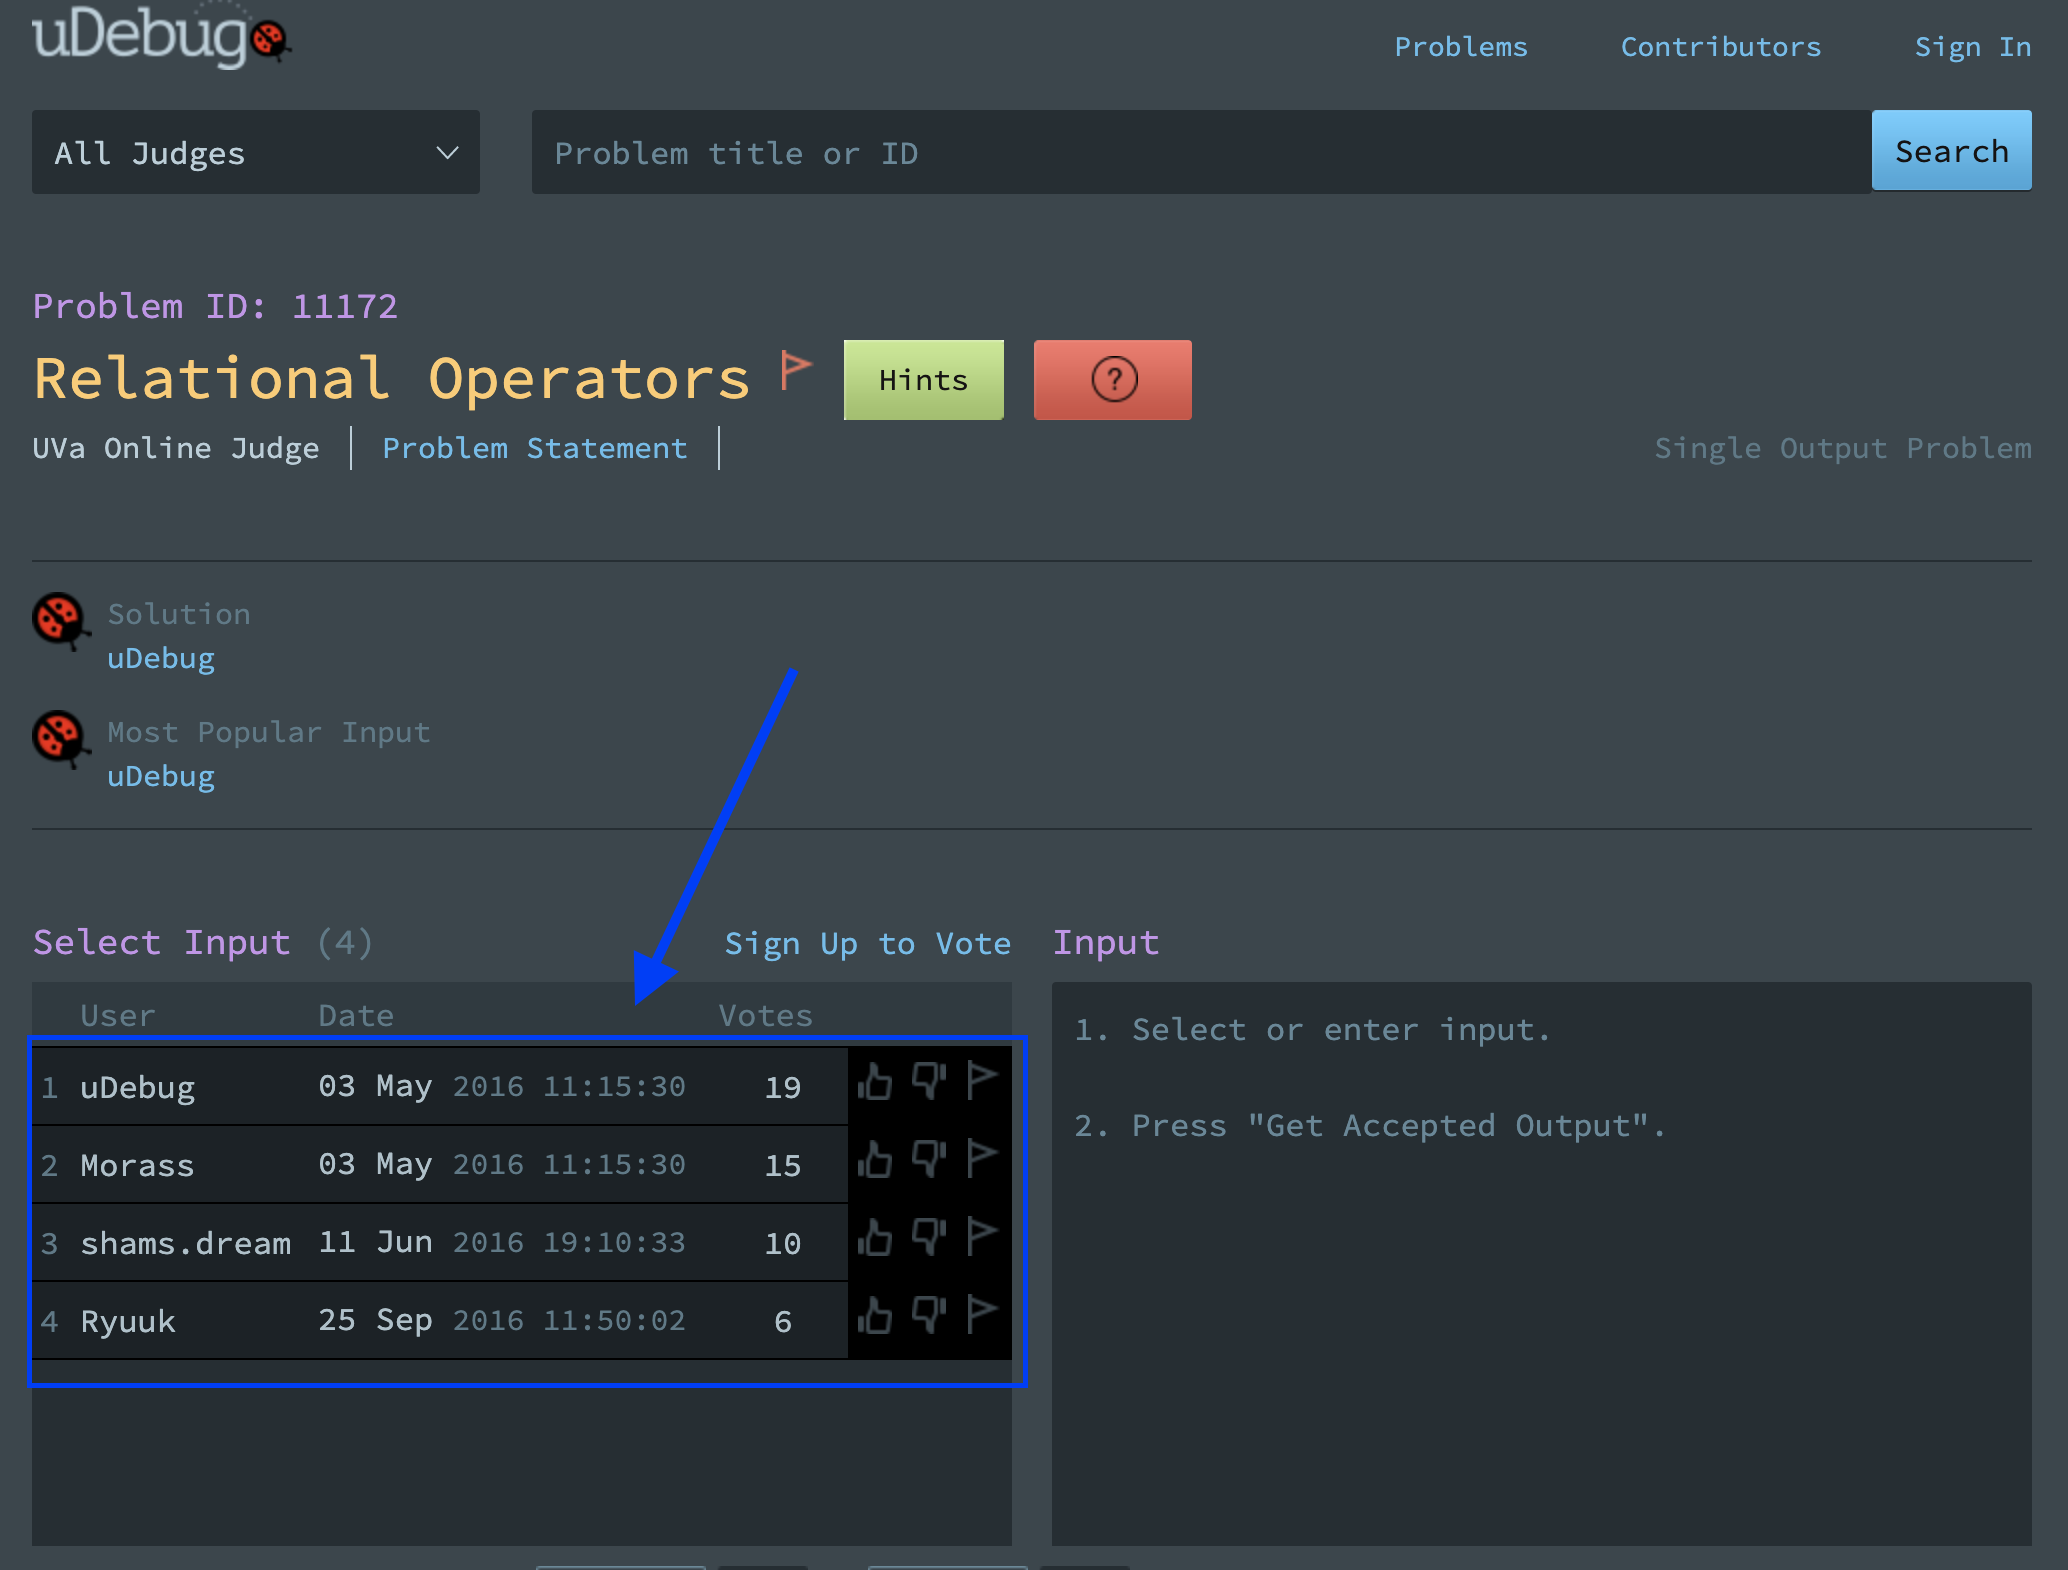
\includegraphics[scale=.4]{images/uhunt_debug_get_data.png}
\end{center}

\hypertarget{pick-a-set}{%
\paragraph{Pick a Set}\label{pick-a-set}}

\begin{enumerate}
\def\labelenumi{\arabic{enumi}.}
\tightlist
\item
  Pick a data set
\item
  Copy it to your clipboard
\end{enumerate}


\begin{center}
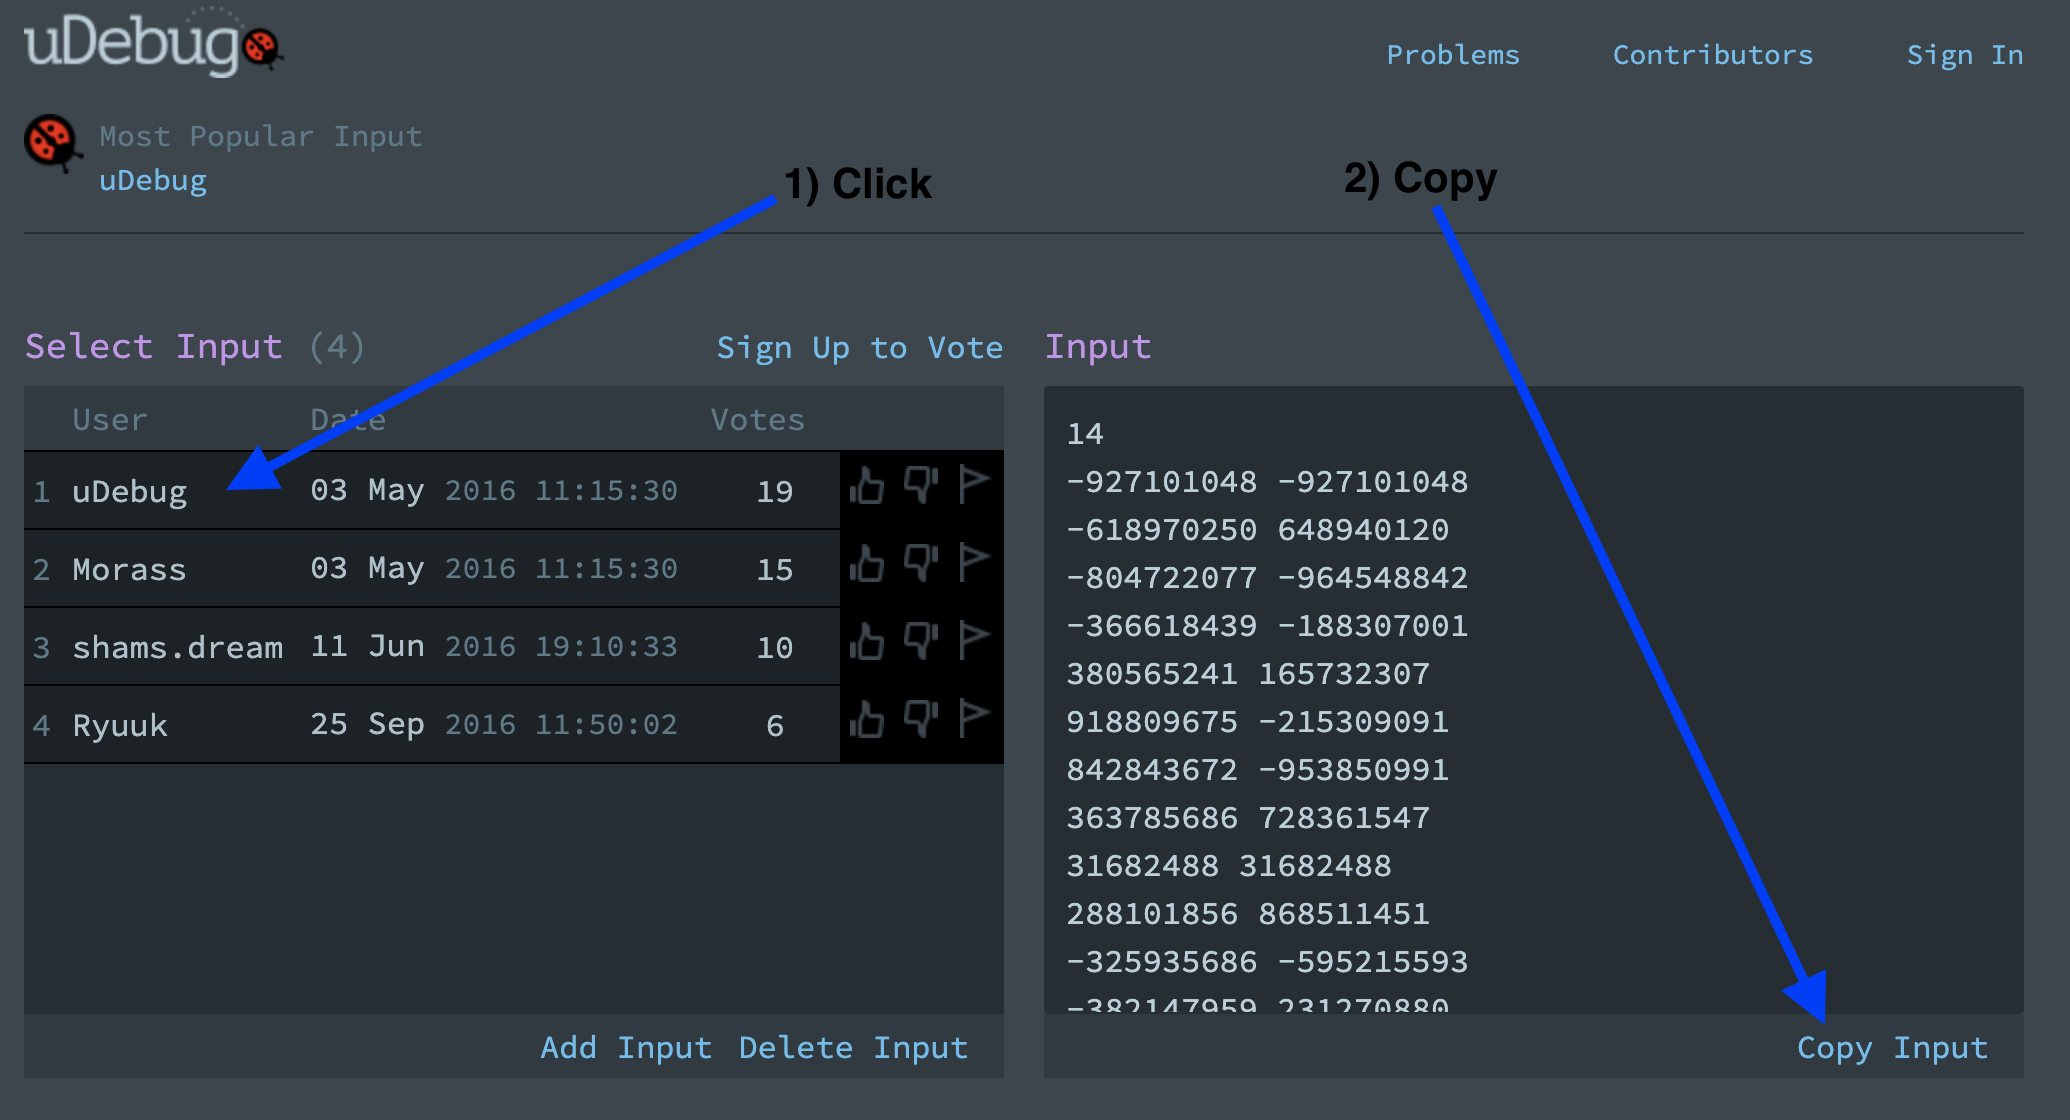
\includegraphics[scale=.4]{images/uhunt_debug_copy_data.png}
\end{center}

\hypertarget{use-new-data}{%
\paragraph{Use New Data}\label{use-new-data}}

\begin{enumerate}
\def\labelenumi{\arabic{enumi}.}
\tightlist
\item
  Create a new file
\item
  Paste new data in file
\item
  Run your code with new data file
\end{enumerate}

\begin{quote}
Your new output will be in the terminal, you need to copy it to bring
back to uDebug.
\end{quote}

\begin{center}
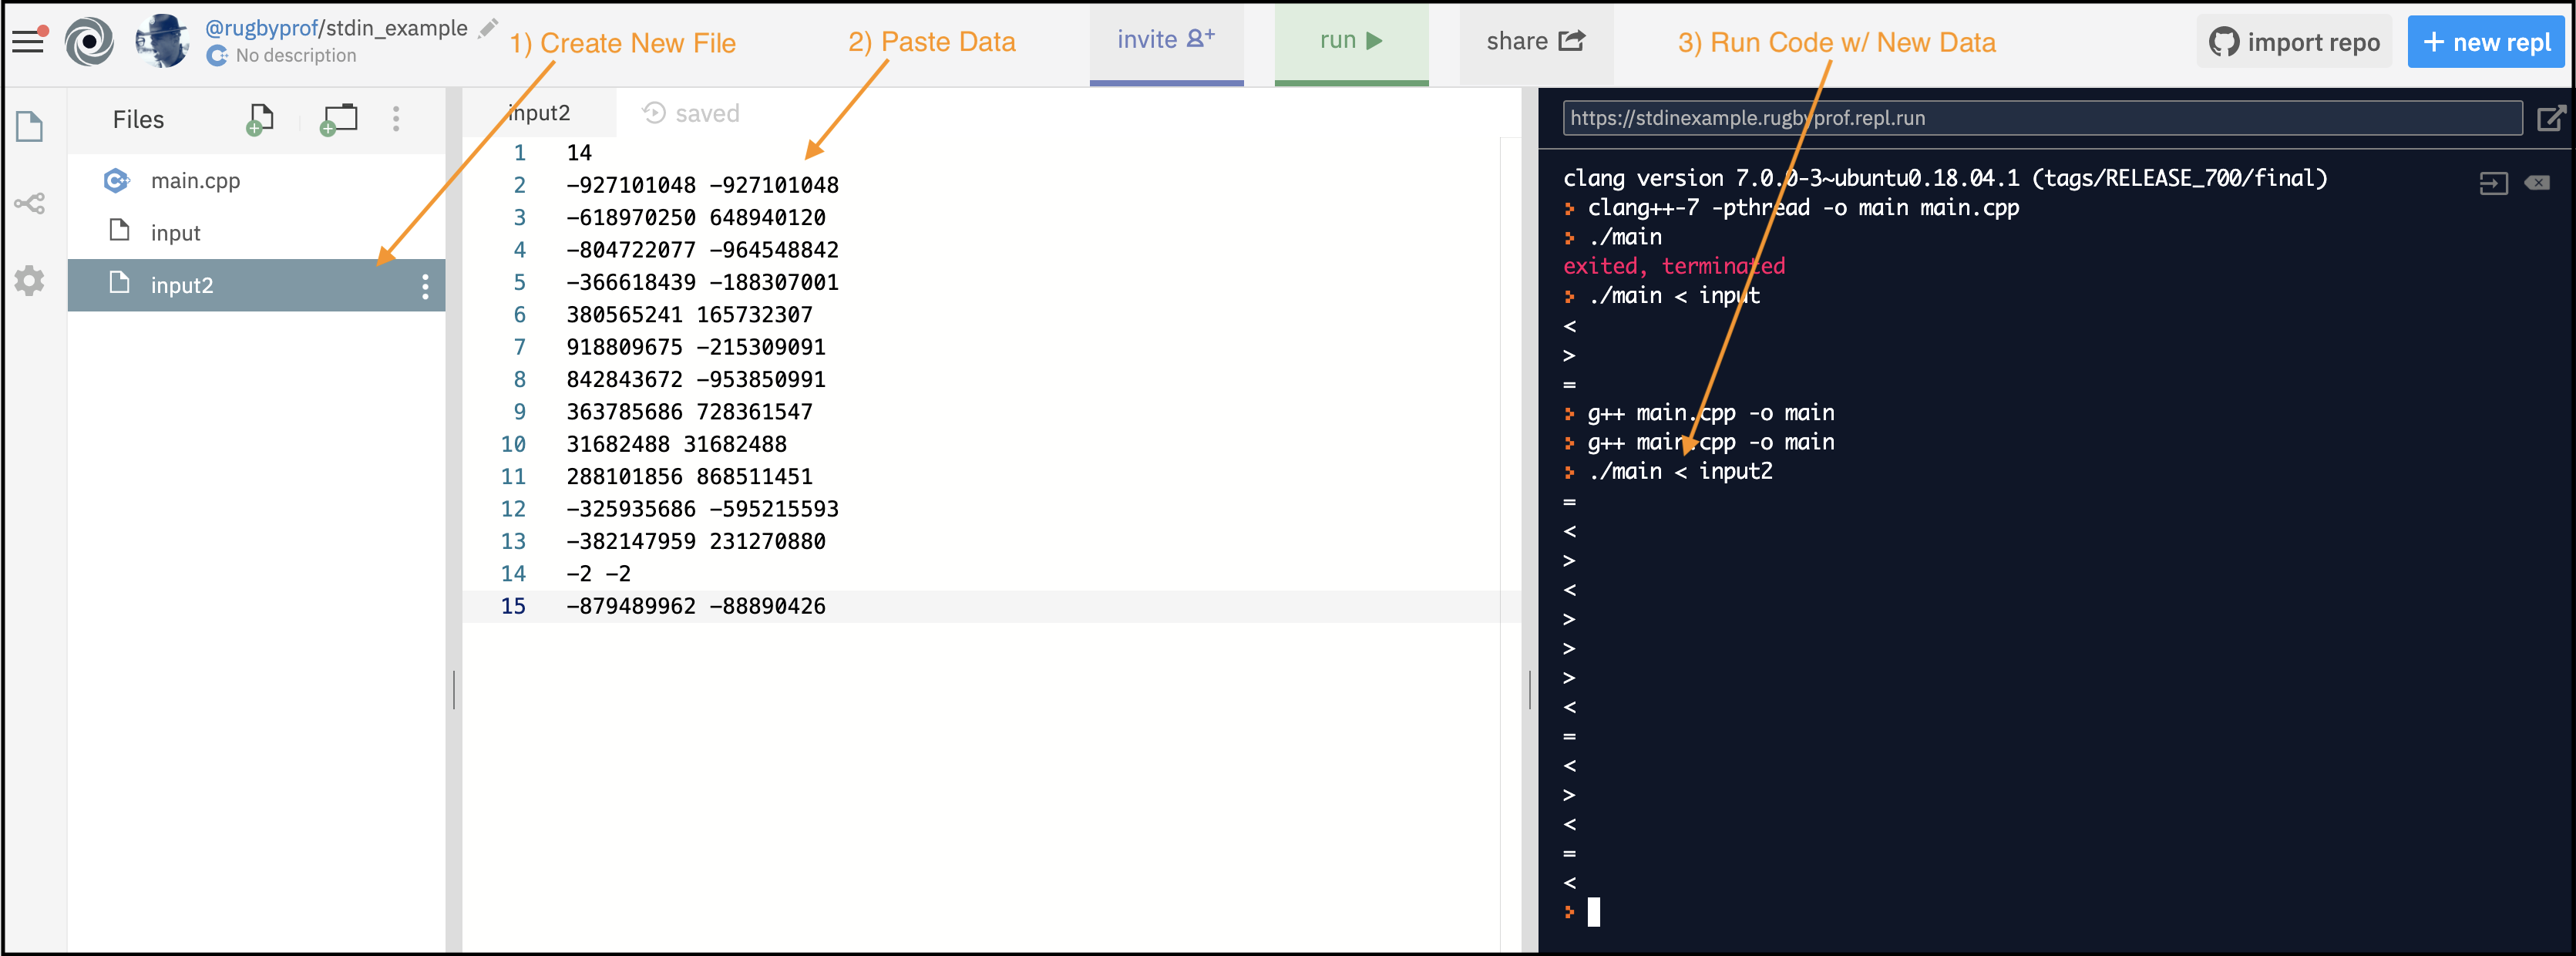
\includegraphics[scale=.3]{images/uhunt_rerun_newdata.png}
\end{center}

\hypertarget{check-new-output}{%
\paragraph{Check New Output}\label{check-new-output}}

\begin{enumerate}
\def\labelenumi{\arabic{enumi}.}
\tightlist
\item
  Click to get accepted output.
\item
  This window shows whats expected.
\item
  This is where you paste your output to be compared with accepted
  output.
\item
  Click to see if it matches!
\end{enumerate}

\begin{quote}
Note: uDebug gives better feedback than simply uploading your solution.
In fact lots of times solutions are rejected for an extra ``newline''.
This can be fixed here at uDebug.
\end{quote}


\begin{center}
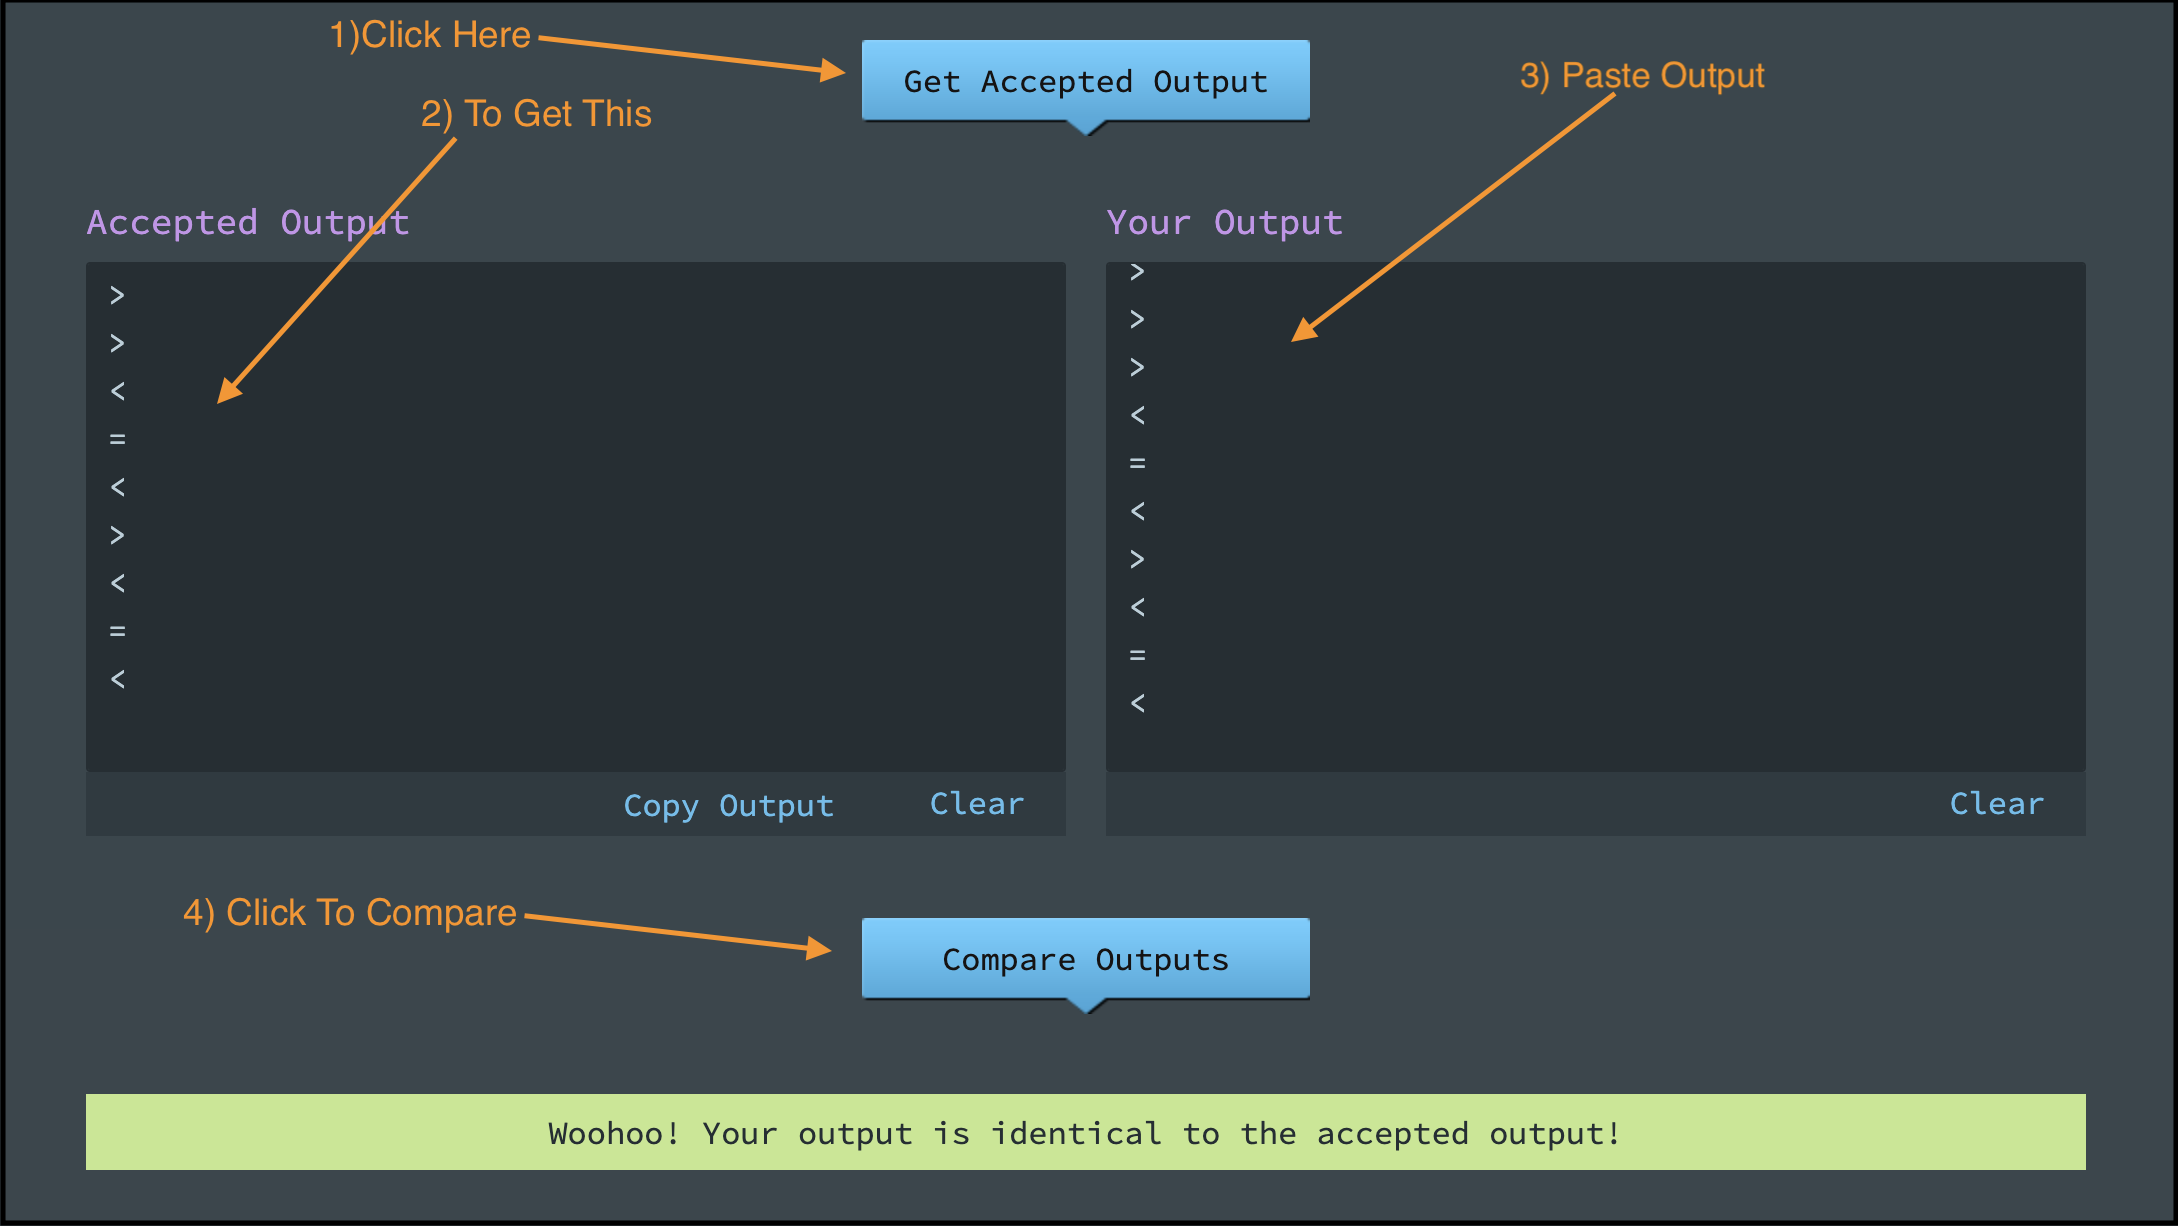
\includegraphics[scale=.4]{images/uhunt_results_newdata.png}
\end{center}

\hypertarget{uploading-solution}{%
\mysubsubsection{Uploading Solution}\label{uploading-solution}}

\hypertarget{start-submission}{%
\paragraph{Start Submission}\label{start-submission}}

\begin{itemize}
\tightlist
\item
  Go back to the problem page and click on submit.
\end{itemize}

\begin{center}
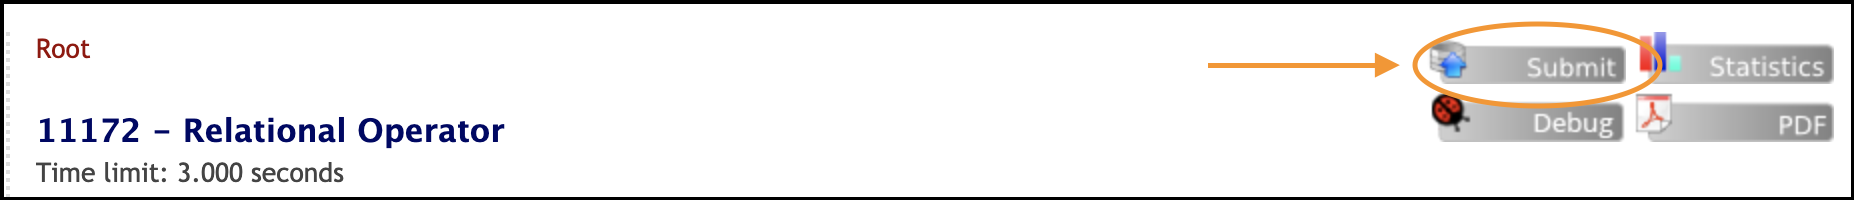
\includegraphics[scale=.4]{images/uhunt_choose_submit.png}
\end{center}

\hypertarget{do-submission}{%
\paragraph{Do Submission}\label{do-submission}}

\begin{itemize}
\tightlist
\item
  On the next page:

  \begin{itemize}
  \tightlist
  \item
    Choose your version of c++
  \item
    Paste your code into the submission text field or Upload a file.
  \item
    Press ``submit''
  \end{itemize}
\end{itemize}


\begin{center}
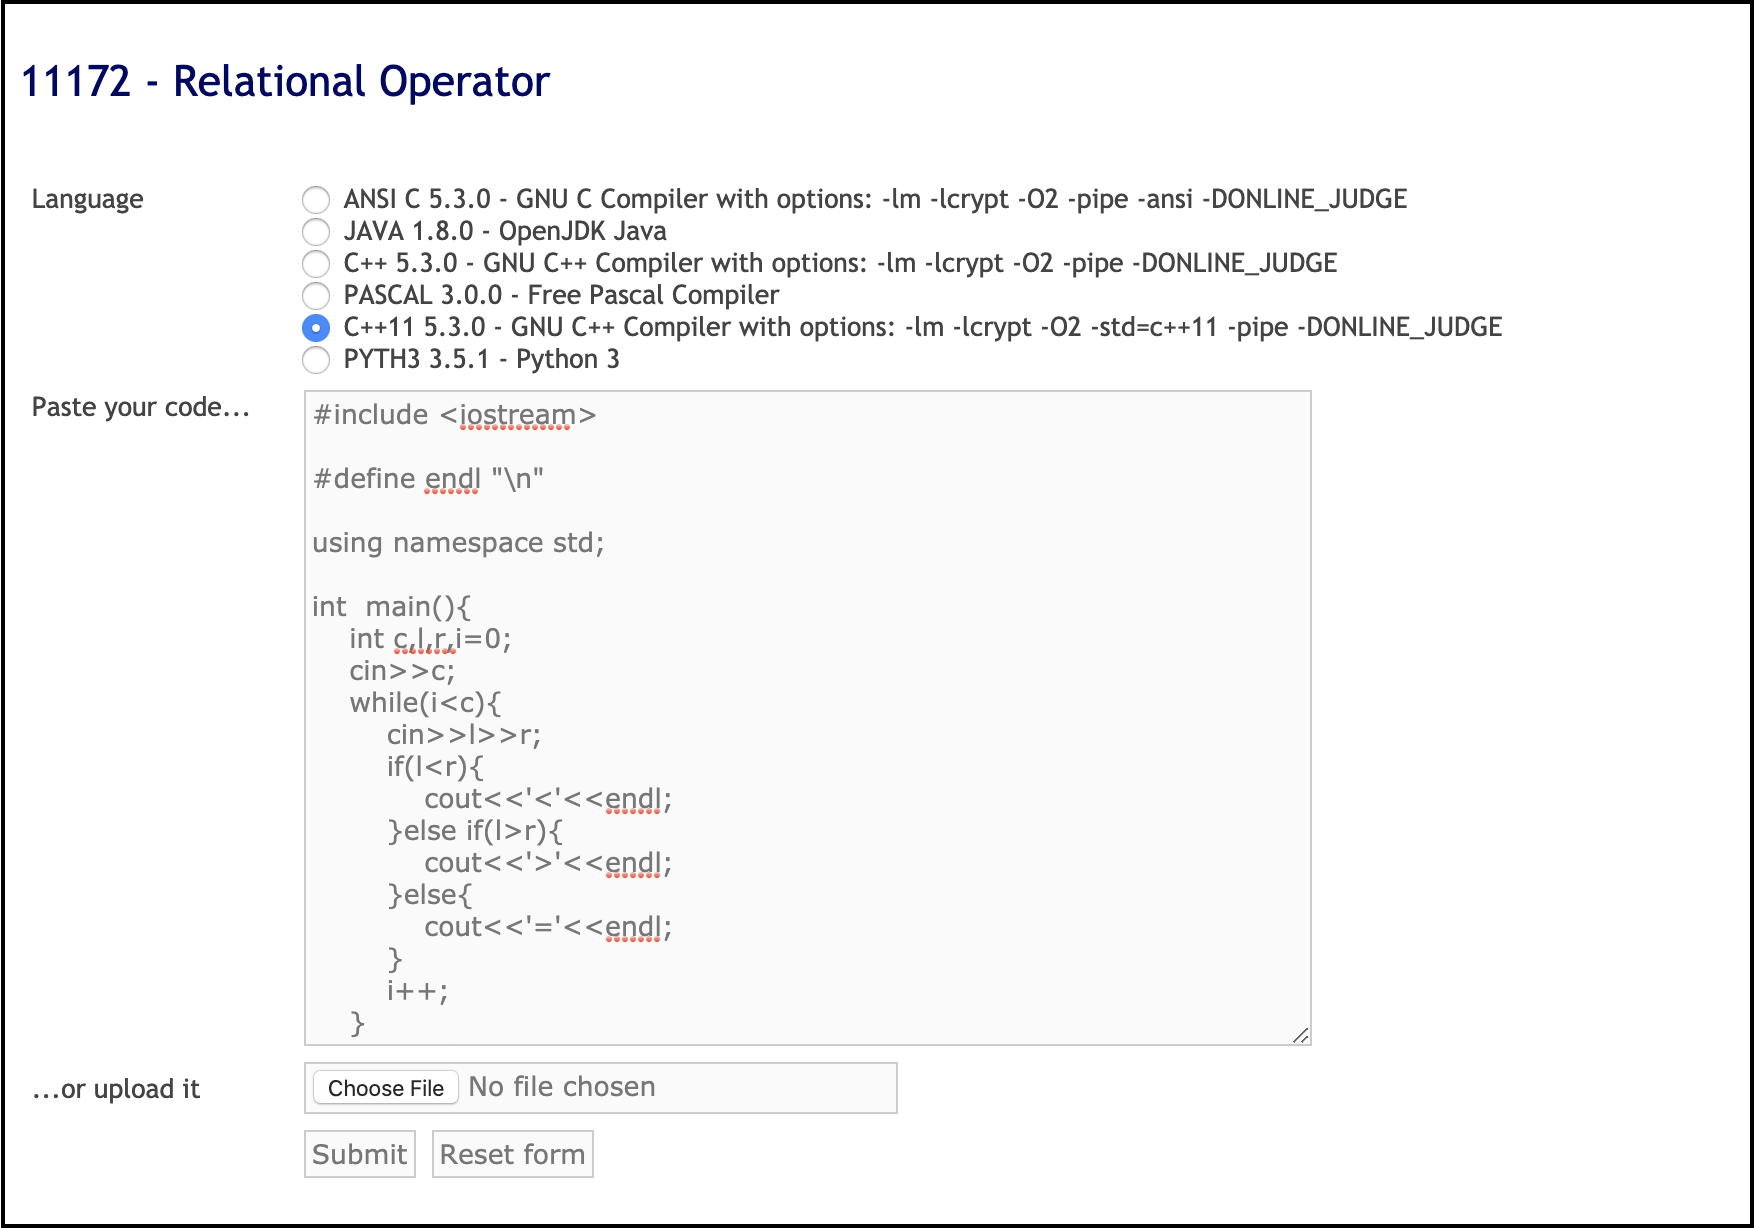
\includegraphics[scale=.4]{images/uhunt_paste_code_submit.png}
\end{center}

\hypertarget{confirm-submission}{%
\paragraph{Confirm Submission}\label{confirm-submission}}

\begin{itemize}
\tightlist
\item
  You Get redirected back to the problem page with a confirmation.
\end{itemize}

\begin{center}
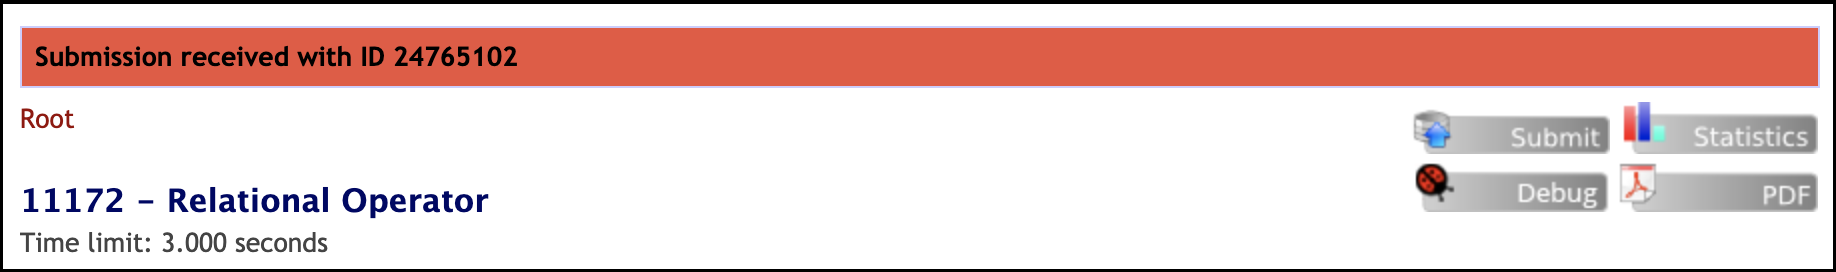
\includegraphics[scale=.4]{images/uhunt_confirm_submit.png}
\end{center}

\hypertarget{submission-results}{%
\paragraph{Submission Results}\label{submission-results}}

\begin{itemize}
\tightlist
\item
  You will get an email telling you what happened, but I like to view
  the stats on the website.
\item
  On the main onlinejudge site.
\item
  Click on last 50 submissions (under site statistics).
\item
  You should see your results (if you don't wait too long).
\end{itemize}

\begin{center}
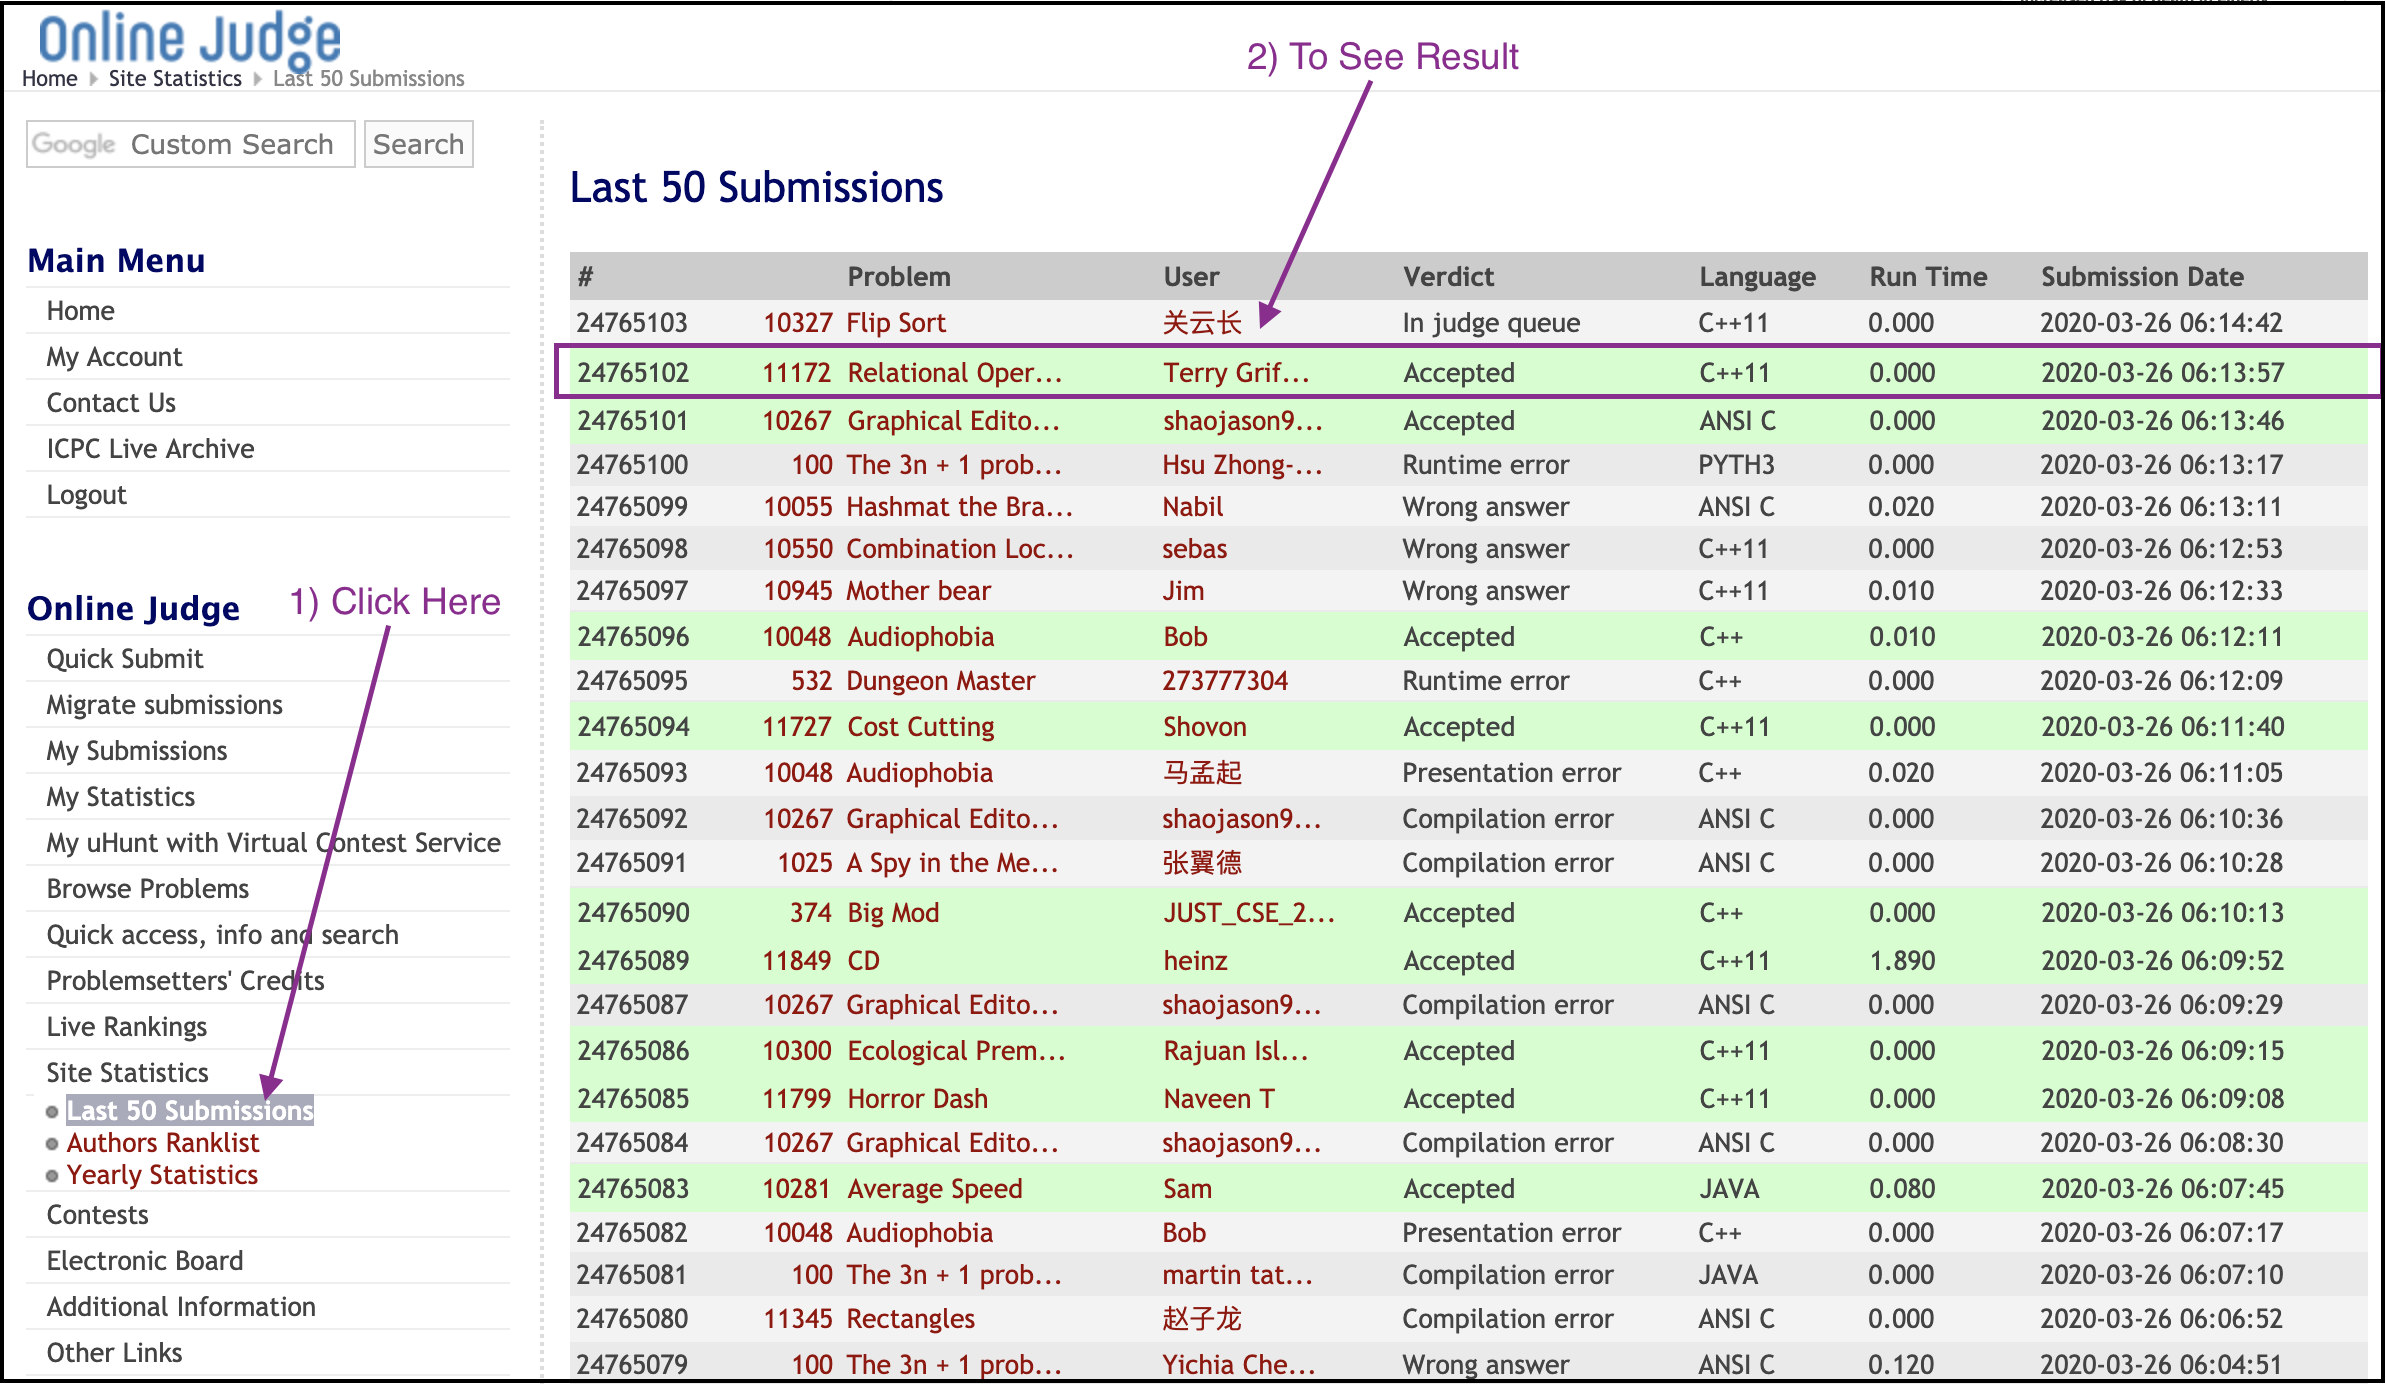
\includegraphics[scale=.4]{images/uhunt_see_results.png}
\end{center}